\documentclass{beamer}
\usepackage{polski}
\usepackage{listings}
\usepackage{ulem}
\usetheme{Dresden}
%\useoutertheme[footline=authortitle,subsection=false]{miniframes}
%\usecolortheme{dolphin}

\author{Piotr Rogula}
\title{Analiza statystyczna czasów na wykonywanie ruchów w
	szachach}
\institute[Pwr]{Politechnika Wrocławska}
\begin{document}
\begin{frame}[plain]
    \maketitle
    \begin{center}
    	pod promotorstwem prof. dr hab. inż. Marcina Magdziarza
    \end{center}
\end{frame}

\section{Wstęp}

\begin{frame}{Spis treści}

\begin{enumerate}
\item wstęp
	\begin{enumerate}
		\item motywacja
		\item kluczowe wyniki innych autorów
		\item potrzebne oznaczenia
	\end{enumerate}
\item wyniki własne
	\begin{enumerate}
		\item sformułowanie problemu
		\item dane
		\item analiza problemu
	\end{enumerate}
\item podsumowanie
\end{enumerate}

\end{frame}

%\begin{frame}{Motywacja}
%\begin{enumerate}
%	\item Szachy jako hobby
%\end{enumerate}	
%\end{frame}
%	\begin{frame}{Motywacja}
%		\begin{enumerate}
%			\item Szachy jako hobby
%			\item popularny temat
%		\end{enumerate}	
%	\end{frame}
		\begin{frame}{Motywacja}
			\begin{enumerate}
				\item Szachy jako hobby
				\item popularny temat
				\item niedosyt literatury opisującej dane zagadnienie
			\end{enumerate}	
		\end{frame}


%%% Kluczowe wyniki innych autorów
\begin{frame}{Kluczowe wyniki innych autorów}
	\begin{itemize}
		\item System Elo \textbf{[cite]} (Arpad Elo)
	\end{itemize}
\end{frame}

\begin{frame}{System Elo}
	\begin{itemize}
		\item przyznawanie punktów bazujące na różnicy rankingu graczy
		\item pierwszy system mający podłoże probabilistyczne
	\end{itemize}
\end{frame}

\begin{frame}{Kluczowe wyniki innych autorów}
	\begin{itemize}
		\item System Elo \textbf{[cite]} (Arpad Elo)
		\item System Glicko-2 \textbf{[cite]} (Mark Glickman)
	\end{itemize}
\end{frame}

\begin{frame}{System Glicko-2}
	\begin{itemize}
		\item ulepszenie systemu Elo.
		\begin{itemize}
			\item wzięcie pod uwagę przedziału ufności rankingu każdego z graczy.
		\end{itemize}
		\item używany w dużej liczbie gier MMO.
	\end{itemize}
\end{frame}

\begin{frame}{Kluczowe wyniki innych autorów}
	\begin{itemize}
		\item System Elo \textbf{[cite]} (Arpad Elo)
		\item System Glicko-2 \textbf{[cite]} (Mark Glickman)
		\item Silnik Stockfish \textbf{[cite]}
	\end{itemize}
\end{frame}

\begin{frame}{Potrzebne oznaczenia}
	\begin{itemize}
		\item \textbf{ruch} składa się z dwóch posunięć - 1 białych i 1 czarnych
			\begin{itemize}
			\item wyjątkiem może być ostatni ruch, gdy po posunięciu białych nastąpił koniec partii.
			\end{itemize}
		\item oznaczenia posunięcia jako ,,błąd'' i ,,duży błąd'' są tożsame
		\item oznaczenie ,,pomyłka'' jest rozróżnialne od oznaczenia ,,błąd'' -- drugie jest wg silnika gorszym posunięciem
	\end{itemize}
\end{frame}


\begin{frame}{Silnik Stockfish}
	\begin{itemize}
		\item funkcja oceny
	\end{itemize}
	wynik liniowej funkcji 
	ważonej sumy cech, na którą składają się między innymi:\\
	$f_b,f_c$ -- wartość figur odpowiednio białych i czarnych\\
	$k_b,k_c$ -- bezpieczeństwo króla odpowiednio białych i czarnych\\
	$m_b,m_c$ -- mobilność figur odpowiednio białych i czarnych\\
	$z_b,z_c$ -- potencjalne zagrożenia wykonane odpowiednio białych i czarnych\\
	\begin{equation*}
		f(f_b,f_c,k_b,k_c,m_b,m_c,\dots)=c_1(f_b-f_c)+c_2(k_b-k_c)+c_3(m_b-m_c)+\dots
	\end{equation*}
	gdzie:
	$c_i$ są stałymi określającymi wagę danej pary zmiennych.
\end{frame}

\begin{frame}{Silnik Stockfish}
	\begin{itemize}
		\item rodzaje błędów szachowych
		\begin{itemize}
			\item ??\hphantom{!} -- błąd (ang. \textit{blunder})
			\item ?\hphantom{?!}  -- pomyłka (ang. \textit{mistake}), posunięcie błędne w mniejszym stopniu niż ,,błąd''
			\item ?!\hphantom{?} -- niedokładność  (ang. \textit{innacuracy}), posunięcie, które można zastąpić zdecydowanie lepszym.
		\end{itemize}
	\end{itemize}
\end{frame}



\section{Wyniki własne}

\begin{frame}{sformułowanie problemu}
	\begin{itemize}
		\item zbadanie zależności pomiędzy czasem poświęconym na wykonanie ruchu, a jego dokładnością
		\item zbadanie zależności między numerem ruchu, a czasem na jego wykonanie oraz jego dokładnością
		\item \sout{próba wyznaczenia optymalnego czasu na wykonanie ruchu\\ minimalizacja ryzyka wystąpienia błędu} 
	\end{itemize}
\end{frame}

\begin{frame}{dane}
	\begin{itemize}
		\item baza danych \textbf{Lichess.com} - 1 plik 72Gb
		\item zbadanie 2 najczęściej granych formatów (600+0, 300+0)
		\item stworzenie bazy ok. 7\% gier ocenionych przez silnik
		\item stworzenie bazy wszystkich ruchów ze wszystkich gier
		\begin{itemize}
			\item 17,52 mln posunięć z 275,94 tyś gier
		\end{itemize}
	\end{itemize}
\end{frame}
\begin{frame}{dane}
		\begin{itemize}
	\item czego nie ma w danych?
		\begin{itemize}
		\item digitalizacja czasu -- czas na posunięcie zaokrąglony do pełnych sekund
		\item brak informacji i odpowiedniej miary dotyczącej sytuacji na szachownicy
	\end{itemize}
	\end{itemize}
\end{frame}


\begin{frame}{dane}
\begin{figure}[H]
	\centering
	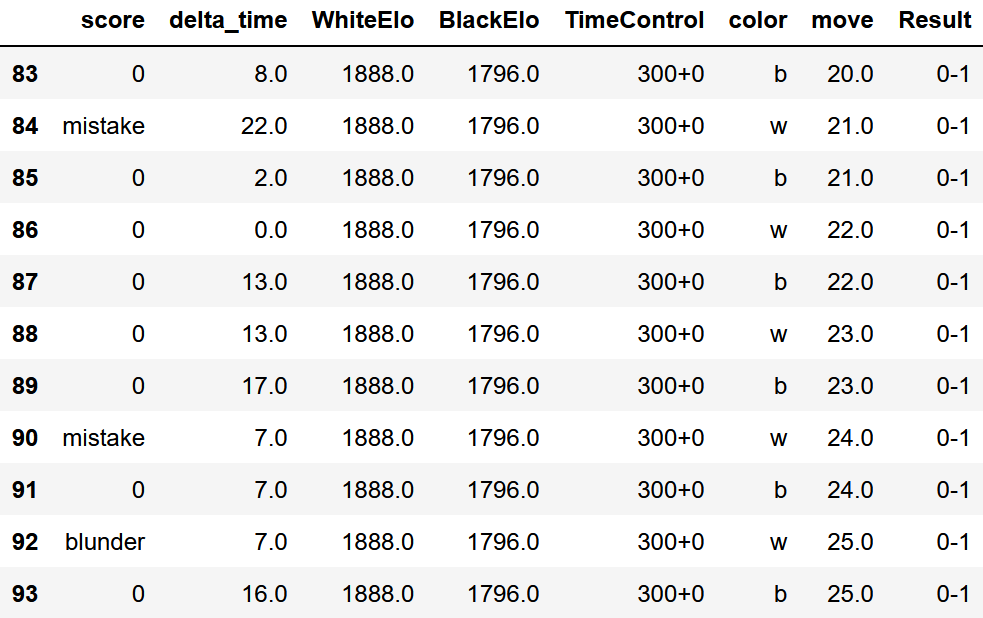
\includegraphics[width=8cm]{../Formatka/danee.png}
	\caption{Fragment bazy zawierającej ruchy z gier o formatach czasowych ,,300+0'' i ,,600+0''.}
	\label{rys:baza_ruchow}
\end{figure}
\end{frame}


\begin{frame}{analiza problemu - wstępny przegląd danych}

	\begin{figure}[H]
		\centering
		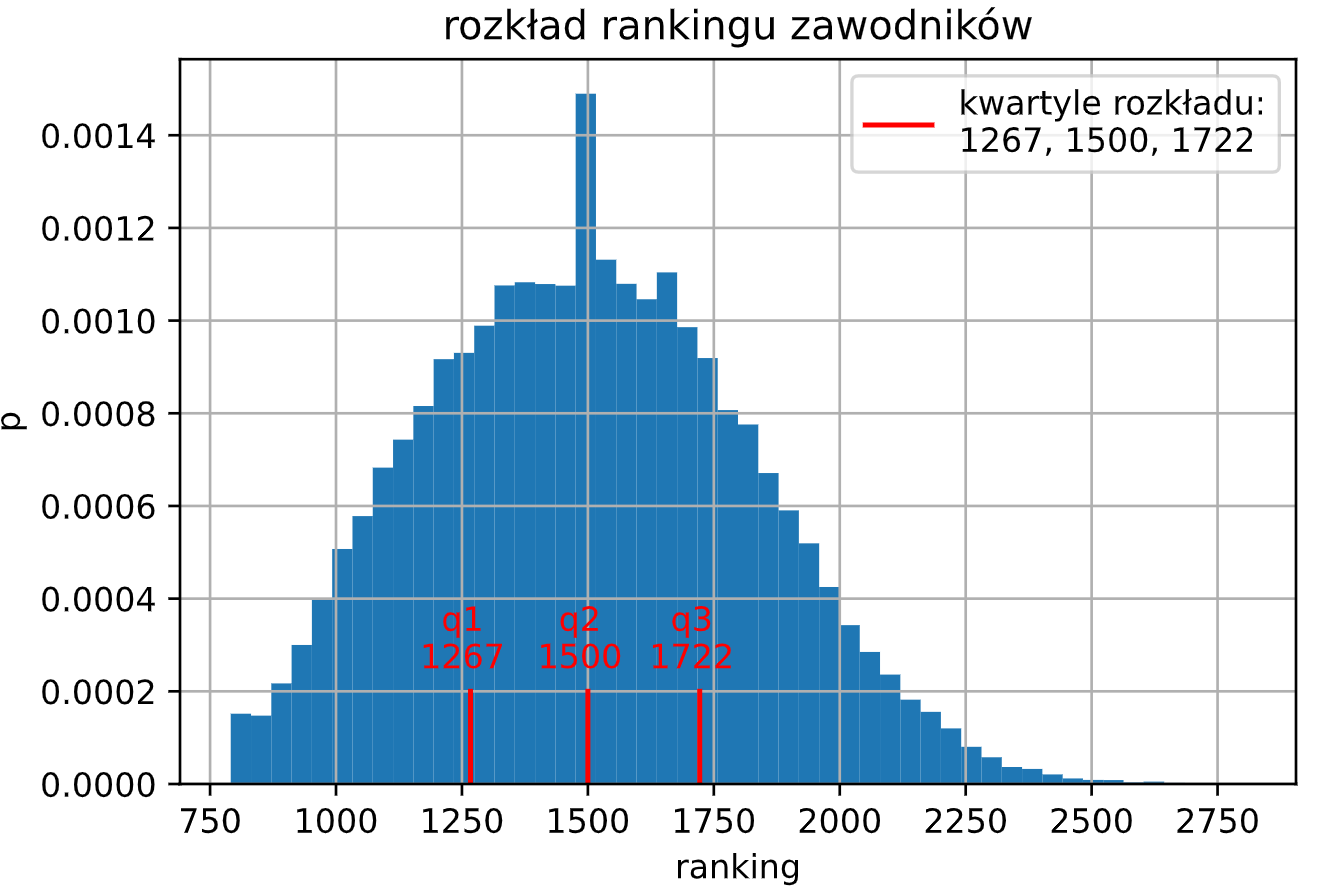
\includegraphics[width=8cm]{../Formatka/ranking.png}
		\caption{rozkład rankingu zawodników wraz z zaznaczonymi kwartylami}
		\label{rys:rozklad_elo}
	\end{figure}
\end{frame}

\begin{frame}{analiza problemu - wstępny przegląd danych}
	\begin{figure}[H]
		\centering
		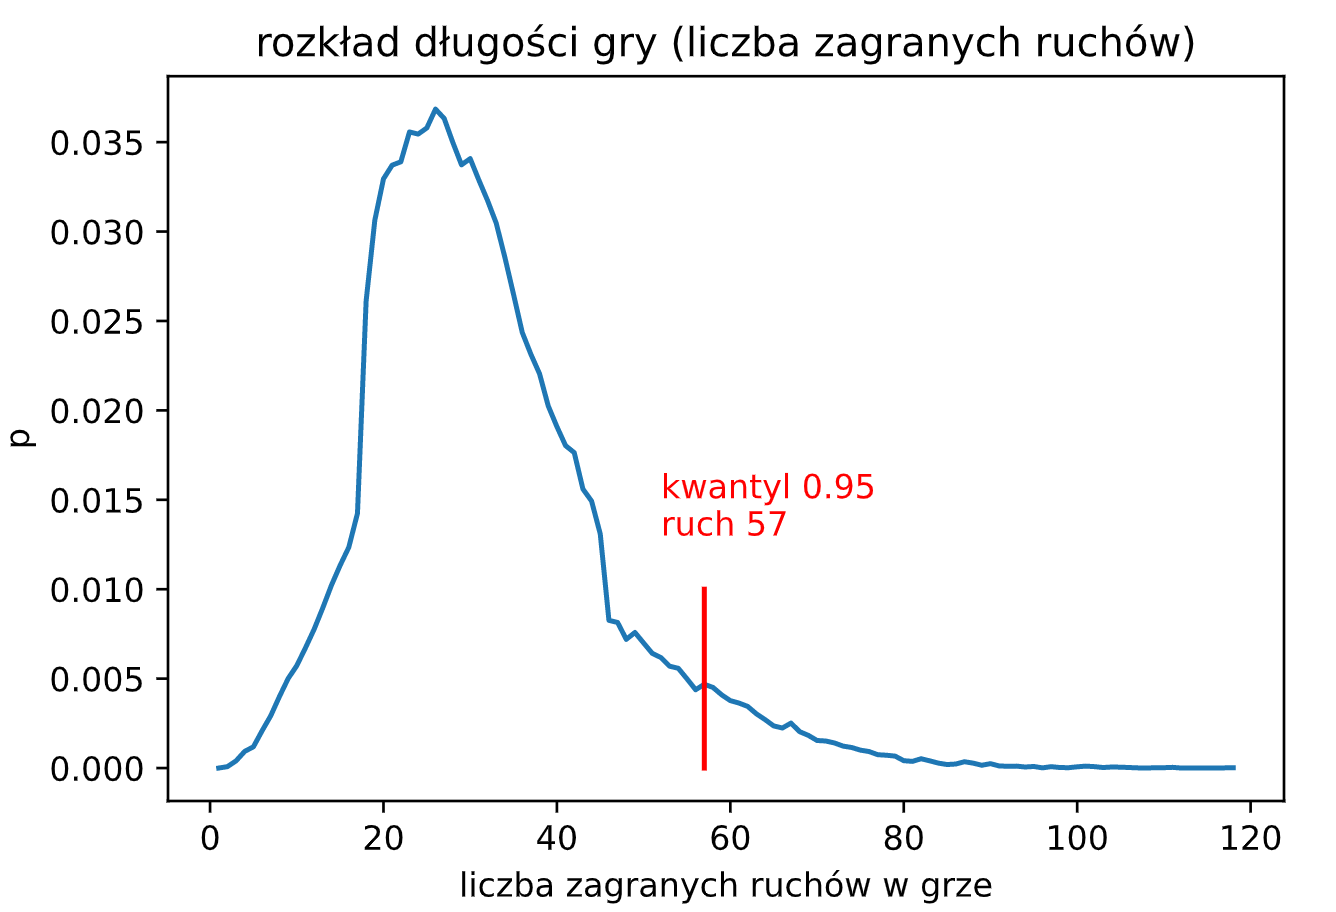
\includegraphics[width=8cm]{../Formatka/dlugosc_gry.png}
		\caption{rozkład długości gier wraz z zaznaczonym kwantylem rzędu 0.95,  dla gier z formatu 300+0 oraz 600+0.}
		\label{rys:dlugosc_gier}
	\end{figure}
\end{frame}




\section{Podsumowanie}

\begin{frame}{Wnioski}
\end{frame}

\begin{frame}{Dalsza praca}
\end{frame}

\begin{frame}{Pytania?}
\end{frame}

\end{document}
